\section{Einführung}\label{sec:einfuhrung}
\subsection{Motivation}\label{sec:motivation}

Bildung ist ein wichtiges Element der Persönlichkeitsentwicklung und unter Artikel 26 der allgemeinen Erklärung der Menschenrechte als solches definiert. Ohne Bildung ist das Ausüben eines gewählten Berufes und das Entwickeln einer Meinung zu komplexen Sachverhalten unmöglich. \cite{weitblicker.org2019:online}. Heute sieht sich Bildung durch den digitalen Wandel der letzten Jahre sich noch nie vorher dagewesenen Problemen gegenübergestellt. Wie können Lehrende an Schulen digitale Technik effizient und preiswert im Unterricht einsetzen und so neue Bildungskonzepte erfolgreich in den Lehrplan integrieren? Ursprünglich bezeichnet der Begriff Digitalisierung das Umwandeln von Analog nach Digital. Wurde früher Musik auf Schallplatten vertrieben, so wurde diese von der Compact Disc vom Markt verdrängt, welche die Musik auf kleinerem Raum digital abspeichert. Auch wenn der Begriff im Zusammenhang mit Schule längst nicht mehr das Ursprüngliche meint, halte ich es für sehr wichtig, früher dagewesene Unterrichtskonzepte nicht einfach zu digitalisieren sondern es erfordert ein Neudenken. Bewährte pädagogische Methoden sollten durch Digitalisierung profitieren sowie neue Konzepte müssen erforscht und entwickelt werden. 

\subsubsection{Besuch Grundschule am Rüdesheimer Platz Berlin}\label{sec:grundschulebesuch}
Im Rahmen der Vorrecherche zu dieser Arbeit wurde einem Unterrichtstag in 
einer Jahrgangsübergreifenden (JüL) Klasse 1 bis 3 an der Grundschule am Rüdesheimer Platz beigewohnt um ein differenzierteres 
Bild der gegenwärtigen Lern- und Digitalisierungssituation an einer Berliner Schule zu bekommen. An dieser Stelle eine große Dankaussagung an Frau Wewer, Grundschullehrerin, welche diese Erfahrung möglich gemacht hat und in einem anschließenden Gespräch das Interesse an einer kostengünstigen und einfach nutzbaren Lösung zur Unterstützung von interaktiven Unterrichtsmethoden unterstrichen hat.
\newpage
\subsection{Problemstellung}\label{sec:problemstellung}
%Kurze Zusammenfassung des Forschungsstandes genügend?
Am 04.04.2019 trat die Änderung des Art. 104c des Grundgesetz für die Bundesrepublik Deutschland in Kraft
und ebnete so den Weg für den von Bund und Ländern beschlossenen Digitalpakt Schule \cite{Art104cG55:online}. 
Dieser Beschluss macht deutlich, dass digitale Kompetenz im Bildungssektor von hoher Bedeutung ist, was auch von einer Förderungssumme von mindestens 5,5 Milliarden Euro unterstrichen wird. 
Legt man diese Summe auf die ca 40.000 Schulen um, erhält jede Schule einen Durchschnittsbeitrag von 137.000 Euro. Bei ca. 11 Millionen Schülerinnen und Schülern würde das eine Förderungssumme von ca. 500 Euro pro Schülerin bzw. Schüler bedeuten. 
Einer der Hauptförderungspunkte des Digitalpakt Schule sieht den Ausbau der technischen Infrastruktur
an deutschen Schulen vor, z.B. Bereitstellung von drahtlosen Netzwerken, schnellen Internetzugangspunkten und digitale Unterrichtsmedien wie interaktive Whiteboards.
\\ \\
Das Bundesministerium für Bildung und Forschung (BMBF) gegenargumentiert damit, dass kein digitales Medium alleine gute Bildung fördert, sondern immer dahinterstehende pädagogische Konzepte aus einer Vielfalt von Angeboten entscheidend sind. \cite{dpakt2019:online} Ergänzend dazu kritisiert Dennis Horn (Experte für digitale Themen der ARD) den zu starken Fokus auf Hardware und mahnt an, dass zu wenig darüber gesprochen wurde, wie diese denn auch sinnvoll genutzt werden kann.\cite{Horn2018:online}. \\ \\
Diese Kritikpunkte wurden auch auf der Podiumsdiskussion der re:publica 2018 - 'Was kommt in den digitalen Schulranzen?' angeschnitten. Tobias Hübner, Lehrer und Autor im Bereich Medienistik, zeigt dort ebenfalls auf, dass der Wille Geld auszugeben zu begrüßen sei, es aber an Konzepten und Materialien mangele. Als Lehrer würde er den Investitionsfokus auf Lehrerfortbildung setzen.
\\ \\

Der populäre Tablet Computer 'iPad' der Firma Apple inc. kostet in der günstigsten Variante bereits mindestens 449€ \cite{iPadmini65:online} (Stand April 2019), was schon knapp 90\% des Förderungsvolumens pro Schülerin und Schüler ausmachen würde. Als ein Gegensatz wäre hier der Einplatinencomputer Raspberry Pi zu nennen, welcher bereits für 33 Euro erwerblich ist (Stand April 2019) und genug Rechenkapazitäten bereitstelle um zahlreiche Projekte im Bildungsbereich durchzuführen. Mit Touchscreenmodul und Schutzhülle liegt der Preis insgesamt bei ca. 150 Euro, was immer noch weniger als die Hälfte des Fördervolumens beträgt. 

\begin{figure}[H]
	\centering
	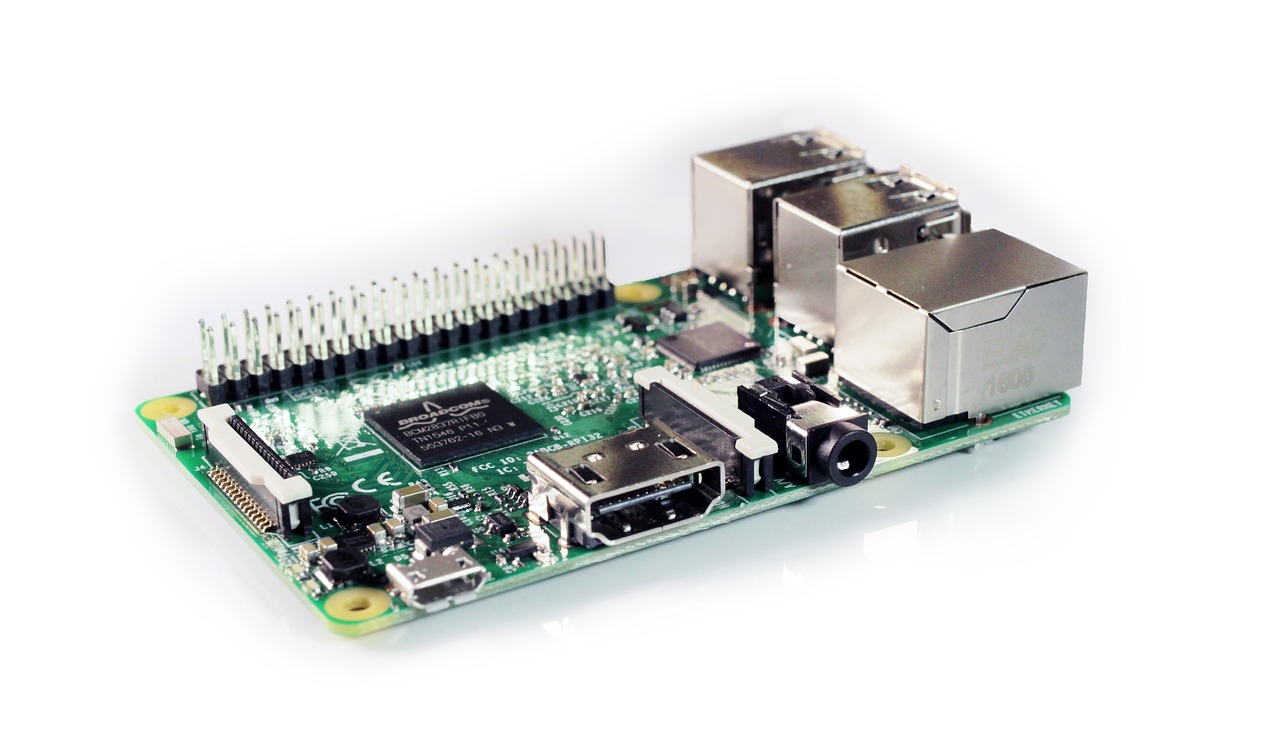
\includegraphics[width=0.8\linewidth]{bilder/raspberry-pi}
	\caption[Raspberry Pi 3 - Einplantinencomputer]{Der Raspberry Pi 3 - Einplantinencomputer \cite{PixaPi2016}}
	\label{fig:server_diagram}
\end{figure}


\subsection{Zielsetzung}\label{sec:zielsetzung}
Seit dem Erfolgskurs des Web 2.0\footnote{Web 2.0 ist ein Schlagwort, das für eine Reihe interaktiver und kollaborativer Elemente des Internets, speziell des World Wide Webs, verwendet wird. Dabei konsumiert der Nutzer nicht nur den Inhalt, er stellt als Prosument selbst Inhalte zur Verfügung. - Wikipedia.org} in den frühen 2000er Jahren, zeichnet sich zunehmend der Trend des Software-as-a-Service Geschäftsmodells ab. Dies beschreibt die Bereitstellung von Software im Internet oder durch ein lokal laufenden Servers, ohne dass Benutzende die Software selbst noch lokal installiert haben müssen. Im Jahr 2015 setzten bereits über drei Viertel von 102 befragten Unternehmen Software dieser Form aktiv im Geschäft ein\cite{TecArt-GmbH2019:online}. Viele Arten von Software können  mittlerweile in einer im Webbrowser lauffähigen Alternative substituiert werden. Ein populäres Beispiel ist die Office-Suite Google Docs der Firma Google inc. Hier lassen sich Textverarbeitung, Tabellenkalkulation und das erstellen von Präsentationen ohne Installation und direkt im Webbrowser des Benutzenden ausführen. Ein anderes Beispiel ist die Web-Software Photopea welche ebenfalls komplett im Web-Browser ausgeführt wird und dem nur lokal installiert ausführbaren quasi Industriestandard Bildbearbeitungsprogramm Photoshop der Firma Adobe inc. sehr nahe kommt. Im Vergleich zu lokal installierter Software ist die Bereitstellung von Web-Software einfacher, da solange ein moderner Webbrowser lauffähig ist, das Betriebssystem des Client-Computers zu vernachlässigen ist. Ebenso stellt potente Hardware keine zwingende Voraussetzungen, da etwaige rechenintensive Aufgaben auf der Serverseite getätigt werden können oder hier eine Balance zwischen Client und Server angestrebt werden kann. \\ 
% Das da oben noch Teil der Problemstellung?
%Hier jetzt Web Trend noch erwähnen!
Ein Raspberry Pi Einplantinencomputer bietet bereits genügend Leistung für Webtechnologien und ein günstigen Anschaffungspreis. Auch besitzen bereits 67\% der 10-11 jährigen Jugendlichen ein Smartphone \cite{Statista2017:online} welches ebenfalls genug Leistung für Webanwendungen aufweisen. \\ \\ Eine Softwarelösung zur Unterstützung von interaktiven Unterrichtsmethoden, welche auf Webtechnologien basiert, könnte den Rahmen der im Digitalpakt Schule fließenden Gelder optimierter ausschöpfen und Schulen finanzielle Flexibilität einräumen. 
\\ \\
Diese Arbeit wird sich der Thematik von pädagogischen digitalen Konzepten und Varianten von interaktiven Unterrichtsmethoden nur im Rahmen der Softwareentwicklung widmen und ihre forschungsrelevante Tiefe nicht gänzlich erfassen, da dies den Rahmen der Zielsetzung überschreiten würde.

%wichtigste Quellen hier noch nennen un
\newpage

\subsection{Aufbau der Arbeit}
Im Anschluss an dieses Kapitel werden \hyperref[sec:grundlagen]{\textbf{Grundlagen}} erörtert. Dies umfasst die Themengebiete Digitalisierung an Schulen und einen Überblick über Webtechnologie. Ersteres ist für den späteren potentiellen Einsatz der Software maßgebend, letzteres bildet das technologische Fundament, welches die Implementierung erst möglich macht. Anschließend wird in Kapitel \hyperref[sec:analyse]{\textbf{Analyse}} ein Vergleich zwischen existierenden kommerziellen und nicht-kommerziellen Plattformen gezogen. Darauf aufbauend folgt eine Anforderungs- und Systembeschreibung. Im darauffolgenden Kapitel \hyperref[sec:konzept]{ \textbf{Konzept}} wird ebendieses erörtert und darauffolgend der Prozess der \hyperref[sec:implementierung]{\textbf{Implementierung}} beschrieben. In einer folgenden \hyperref[sec:auswertung]{\textbf{Auswertung}} werden die Ergebnisse mit den geplanten Zielen verglichen und ein Fazit gezogen. Schlussendlich wird im letzten Abschnitt ein \hyperref[sec:ausblick]{\textbf{Ausblick}} formuliert, welcher die Zukunft des Projekts betrifft. 
   
